\chapter{Deep Learning}

\section{Interview of Fame}

\subsection{Geoffrey Hinton}
\subsubsection{Knowledge Embedding}
\begin{itemize}
	\item BP
	\begin{itemize}
		\item psychology view: knowledge in vectors
		\item semantic AI: knowledge graph
		\item BP algorithm can interpret \& convert between feature vector and graph representation (with some embedding)
	\end{itemize}
	\item Boltzmann Machine
	\begin{itemize}
	\item Leaning Algorithm on Density Net
		\begin{itemize}
		\item same information in forward \& backward propagation to learn feature embedding
		\end{itemize}
	\item Restricted Boltzmann Machine (RBM)
		\begin{itemize}
		\item ways of learning in deep dense net with fast inference
		\item iterative learning (adding layer after the above trained)
		\item ReLU $\Leftrightarrow$ a stack of sigmoid functions (approximately) in RBM
		\item ReLU units initialized to identity for efficient learning
		\end{itemize}
	\end{itemize}
	
	\item EM
		\begin{itemize}
		\item EM with Approximate E Step
		\end{itemize}
	
	\item vs. Symbolic AI
		\begin{itemize}
		\item Symbolic AI: symbolic logic-like expression to do reasoning
		\item yet, maybe state vector to represent knowledge
		\end{itemize}
\end{itemize}

\subsubsection{Brain Science}
\begin{itemize}
\item Brain: Nets Implemented by Evolution
	\begin{itemize}
	\item trying to train without BP
	\item doing BP (get derivatives) with re-construction error (auto-encoder)
	\end{itemize}
\end{itemize}

\subsubsection{Memory in Nets}
\begin{itemize}
\item Fast Weights for Short-term Memory
\item Capsule Net
	\begin{itemize}
	\item structured knowledge representation in each unit (feature with sets of property)
	\item $\Rightarrow$ enable nets to vote rather than filtering - thus better generalization
	\end{itemize}
\end{itemize}

\subsubsection{Unsupervised Learning}
\begin{itemize}
\item Importance
	\begin{itemize}
	\item better than human eventually (as supervised learning has limited maximum)
	\item GAN as a breakthrough
	\end{itemize}
\end{itemize}

\subsubsection{"Slow" Feature}
\begin{itemize}
\item Non-linear Transform to Find Linear Transform
	\begin{itemize}
	\item find a latent representation containing linear transform to do the work
	\item e.g. change viewpoints: pixels $\rightarrow$ coordinates $\rightarrow$ linear transform $\rightarrow$ back to pixels
	\end{itemize}
\end{itemize}

\subsubsection{Relations between Computers}
\begin{itemize}
\item showing computer data to work
	\begin{itemize}
	\item instead of programming it to work
	\end{itemize}
\end{itemize}


\subsection{Pieter Abbeel}
\subsubsection{Deep Reinforcement Learning}
\begin{itemize}
\item Overall Challenge 
	\begin{itemize}
	\item Representation
	\item Exploration Problem
	\item Credit Assignment
	\item Worst Case Performance
	\end{itemize}
\item Advantage (Deep Nets in RL)
	\begin{itemize}
	\item network capturing the representation (state vector)
	\end{itemize}
\item Question in DRL
	\begin{itemize}
	\item how to learn safely
	\item how to keep learning (under small negative samples) e.g. better than human
	\item can we learn the reinforcement learning program (RL in the RL)
	\item long time horizon
	\item use experience across tasks
	\end{itemize}
\item Success of DRL
	\begin{itemize}
	\item simulated robot inventing walking... $\Rightarrow$ single general algorithms to learn
	\end{itemize}
\end{itemize}

\subsection{Research Advices}
\begin{itemize}
	\item Reading
	\begin{itemize}
		\item read a little bit \& find somewhere intuitively not right
		\begin{itemize}
			\item good intuition: eventually work; bad intuition: not working no matter what it is doing
			\item if other doubts your idea as bullshit $\Rightarrow$ a sign for real good result
		\end{itemize}
		\item a supervisor with similar belief
		\item PhD vs. Company
			\begin{itemize}
			\item amount of mentoring
			\item faster if dedicated supervisor available
			\end{itemize}
	\end{itemize}
	
	\item Practice
		\begin{itemize}
		\item open-source learning resource
		\item implement the paper
		\end{itemize}
\end{itemize}


\section{Basic Neutral Network}

\subsection{Goal and Advantages}
\subsubsection{Data Mining and Pattern Recognition}
\begin{itemize}
\item Larger Maximum Capability
	\begin{itemize}
	\item Curve given Amount of Data
	\begin{figure}[ht]
	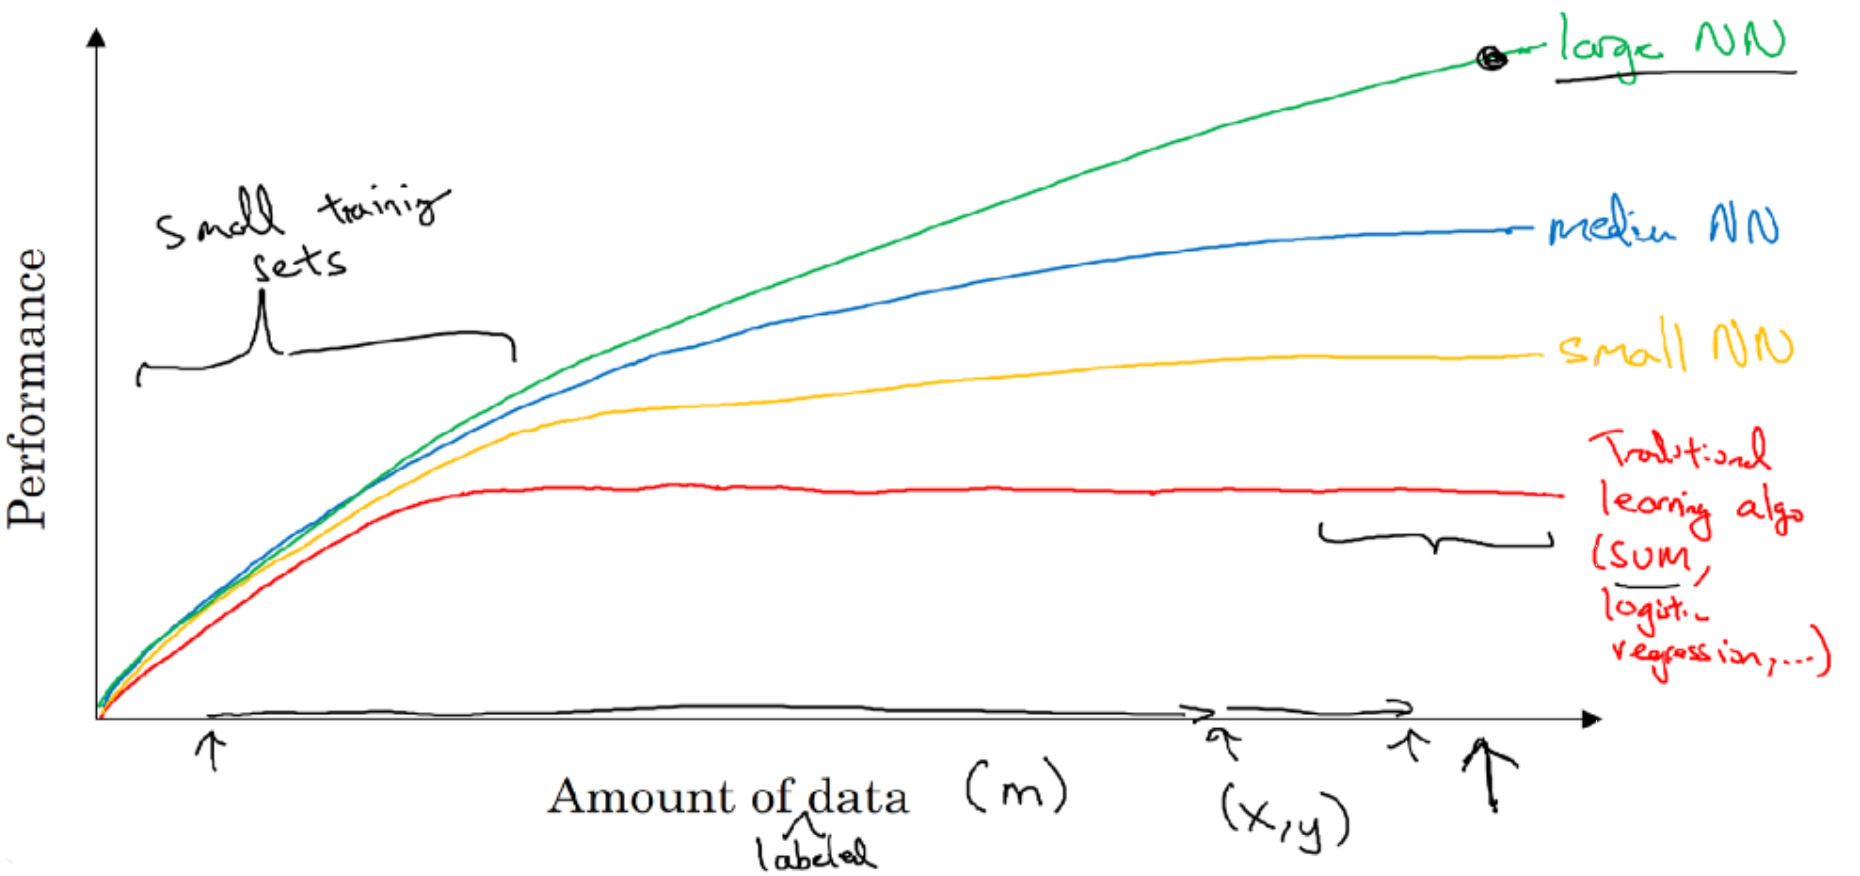
\includegraphics[width=\linewidth]{./Deep Learning/background-largedata.png}
	\end{figure}
	\item Reasons
		\begin{itemize}
		\item the scale of data (labeled)
		\item the scale of neural network (computability)
		\item the scale of efficiency: e.g. ReLu, faster parallel algorithm
		\end{itemize}
	\end{itemize}
\end{itemize}

\subsubsection{Ability to Choose}
\begin{itemize}
\item Choosing Basis Functions
	\begin{itemize}
	\item Functional View
		\begin{itemize}
		\item $\displaystyle y(\mathbf {x}, \mathbf w)=f(\mathbf w^T\phi(\mathbf x)), \text{ where } \phi \text{ is basis function }, f(\cdot) \text{ is net as a function}$
		\end{itemize}
	\item Learning $\phi$: choose embedding $\Rightarrow$ choose basis function
	\item Learning $\mathbf w$: choose which feature / basis functions more useful
	\end{itemize}
\end{itemize}

\subsection{Problem}
($n$ units in one hidden layer)

\subsubsection{Weight-space Symmetries} 
\begin{itemize}
\item Symmetries in Activation Function
	\begin{itemize}
	\item $\mathcal{O}(2^n)$, e.g. $\arctan(-x) = -\arctan(x) \Rightarrow$ changing signs of all input \& output has the same mapping (reduce effective data)
	\end{itemize}
\item Positional Combination in One Layer
	\begin{itemize}
	\item $\mathcal{O}(n!)$ exchange unit with each other (together with their input output weights) $\Rightarrow$ mapping stay the same
	\end{itemize}
\end{itemize}
$\Rightarrow \mathcal O(n!2^n)$ overall weight-space symmetries

\subsubsection{Non-convex Error Function}
\begin{itemize}
\item Multiple Critical Points
	\begin{itemize}
	\item at least $\mathcal O (n!2^n)$ critical points ($\nabla E(w) = 0, \text{ where } E(w) \text{ is error function}$) due to weight-space symmetries
	\end{itemize}
\item Expensive in Finding Critical Point
	\begin{itemize}
	\item expensive for even local optima with gradient decent
	\item as expensive as $\mathcal O(n^3)$ if using Laplace approximation
	\end{itemize}	
\end{itemize}

\subsubsection{Gradient Vanishing}
\begin{itemize}
\item Ability of Depth (however)
	\begin{itemize}
	\item functions that can be compactly represented by a depth $k$ architecture might require an exponential number of computational nodes using a depth $k-1$ architecture
	\end{itemize}
	
\item Possible Solutions
	\begin{itemize}
	\item Xavier initialization, ReLU activation, ...
	\end{itemize}	
\end{itemize}

\subsection{Learning}
\subsubsection{Forward-Backward Propagation}
\begin{itemize}
\item Representation
	\begin{itemize}
	\item Layers
		\begin{itemize}
		\item input layer, hidden layer(s) (each has a bias term $x_0=1$)
		\item output layer
		\end{itemize}
	\item Neuron (Unit)
		\begin{itemize}
		\item $s_l$: num of units in layer $l$
		\item $w^l$: weight matrix of mapping from layer $l$ to $l+1$, with shape of $s_{l+1}, (s_l + 1)$
		\item $a_j^l$: activation of unit $j$ at layer $l$
		\item $h(\cdot)$: activation function (usually shared)
		\item $z_j^l$: output of unit $j$ at layer $l$ (represent parameterized basis)
		\end{itemize}
	\end{itemize}
\item Forward Propagation
	\begin{itemize}
	\item Activation $a^{j+1} = w^j \cdot [z_0^j, ..., z_{s_j}^j]^T, \text{ with } z_0=1$
	\item Unit Output $z^{j+1} = h(a^{j+1}) = [z_1^{1}, ..., z^{j+1}_{s_{j+1}}]^T$
	\end{itemize}

\item Backward Propagation
	\begin{itemize}
	\item
	\end{itemize}

\end{itemize}


\subsubsection{}

\section{Advanced Topic}
\subsection{Machine Reading Comprehension}
\subsubsection{Problem Formulation}
\begin{itemize}
\item 
\end{itemize}

\subsubsection{RNN with Attention}
\subsubsection{Convolution with Self-attention - QAnet}
\begin{itemize}
\item 
\end{itemize}